\documentclass[a4paper, 10pt]{article}
\usepackage{amsmath}
\usepackage{amsfonts}
\usepackage{amssymb}
\usepackage{braket}
\usepackage{graphicx}
\usepackage{booktabs}
\usepackage{caption}
\usepackage{graphicx}
\usepackage{float}
\usepackage{wrapfig}
\renewcommand{\figurename}{Figura}
\renewcommand\refname{Materiale consultato}
\renewcommand{\abstractname}{}
\usepackage{listings}
\usepackage{gensymb}
\usepackage{verbatim}
\usepackage{hyperref}
%\usepackage{lmodern}
\hypersetup{%
	colorlinks=false,
	linkbordercolor={0 1 0},
	pdfborderstyle={/S/U/W 1},
	linkcolor=blue,
	urlcolor=blue
}
\newcommand{\reff}[1]{\mbox{\ref{#1}}}
\usepackage[sc]{mathpazo}
\linespread{1.03}         % Palladio needs more leading (space between lines)
\usepackage[T1]{fontenc}


\title{\textbf{Metodo Perturbativo Stazionario}}
\author{Paul Butuc \\ Universita' degli Studi di Torino}
\date{2019}


\begin{document}
\pagenumbering{roman}
\maketitle
\vfil

\begin{abstract}
In questo saggio si tratta la teoria perturbativa, uno dei tre principali metodi di risoluzione approssimata in meccanica quantistica nel caso di sistemi fisici reali. Si farà riferimento alla rappresentazione di Schr\"odinger e si svilupperà il metodo per trovare soluzioni approssimate dell'equazione agli autovalori per l'hamiltoniana di un sistema incognito $H\ket{\phi} = E\ket{\phi}$ usando le soluzioni esatte del sistema noto $H_0\ket{\phi}^{(0)} = E^{(0)}\ket{\phi}^{(0)}$. Verrà considerato il caso in cui $H$ e $H_0$ non dipendono dal tempo e lo spettro di $H_0$ è discreto e non degenere.
\end{abstract}
\newpage
\pagenumbering{arabic}


%%
\section{Introduzione}
\begin{small}
La formulazione moderna della meccanica quantistica è incentrata sul concetto fondamentale di funzione (o vettore) di stato ed una serie di relativi postulati.

Ogni sistema fisico è caratterizzato in ogni istante della sua evoluzione, da una specifica funzione di stato (tralasciando la matrice densità e le relative miscele statistiche). Nella sua forma più generale la funzione di stato (puro) $\psi$, è un vettore in un certo spazio (funzionale) di Hilbert $\mathbb{H}$ e contiene tutta l'informazione disponibile riguardo il sistema fisico che rappresenta. $\psi$ ha un'interpretazione probabilistica: fornisce la distribuzione di probabilità dei valori risultanti da qualunque misura effettuata sul sistema.

Le osservabili della fisica classica diventano operatori hermitiani \^A (in genere non limitati) sullo spazio $\mathbb{H}$. Gli operatori agiscono sul vettore di stato fornendo il risultato (aleatorio o meno) della misura di una certa grandezza. In particolare, l'equazione agli autovalori, fornisce (con probabilità 1) tutti i valori possibili dell'osservabile nei relativi stati.

Secondo queste ipotesi, conoscere completamente un sistema dal punto di vista quantistico consiste nel determinare l'evoluzione degli operatori e/o vettori di stato nel tempo. Nella rappresentazione di Schr\"odinger si avrà $\psi = \psi(t), \textnormal{\^A} = cost.$, in quella di Heisenberg, $\psi = cost., \textnormal{\^A} = \textnormal{\^A(t)}$.

Nella rappresentazione di Schr\"odinger il vettore di stato diventerà la nota funzione d'onda $\psi = \psi(\vec{r} , t)$, dipendende dalle coordinate e dal tempo. In questo caso l'evoluzione temporale del sistema è data dall'equzione di Schr\"odinger dalla quale si può ricavare un'operatore di evoluzione temporale $U(t,t_0)$ che, applicato a $\psi(\vec{r}, t_0)$ fornisce $\psi(\vec{r}, t)$ per qualunque $t$.

Nel nostro caso l'hamiltoniana $H$ del sistema non dipende dal tempo (caso stazionario), e il problema di ricavare $U(t, t_0)$ si riduce alla soluzione dell'equazione agli autovalori per $H$. Bisogna quindi saper risolvere l'equazione differenziale associata. Putroppo però la soluzione esatta è, nella maggior parte dei casi reali, impossibile (con le tecniche matematiche note).

Si rende quindi necessario sviluppare dei metodi di approssimazione delle soluzioni per tutti i casi in cui non si può arrivare alla soluzione esatta. Fra gli svariati metodi esistenti se ne possono distinguere alcuni abbbastanza generici da essere studiati in modo sistematico ed applicati ad una classe sufficientemente ampia di sistemi.

Fra questi i tre principali sono: il metodo WKB per sistemi approssimabili a sistemi classici (dove $\hbar \rightarrow 0$). Il metodo variazionale, utile per stimare l'energia dello stato fondamentale del sistema. Infine, \textbf{il metodo delle perturbazioni stazionarie}, trattato in questo saggio.
\end{small}


%%
\section{Descrizione generale}
Si consideri il sistema descritto dall'hamiltoniana $H_0$ e la relativa equazione agli autovalori:
\begin{equation}
	\label{sistema-noto-full}
	H_0\ket{\phi_n^{(0)} \alpha} = E_n^{(0)}\ket{\phi_n^{(0)} \alpha}
\end{equation}
dove lo $zero$ indica che ci si riferisce al sistema noto, mentre $\alpha$ tiene conto del caso più generale in cui il sistema potrebbe avere livelli di energia degeneri.

Si supponga che il sistema sia risolvibile in modo esatto. Questo significa che si è in grado di ottenere l'insieme di tutti gli autovalori $\{E_n^{(0)}\}$ ed il relativo insieme completo ed ortonormale di autofunzioni $\{\ket{\phi_{n}^{(0)}\alpha}\}$.

Si supponga inoltre che gli autostati siano correttamente normalizzati: 
\begin{equation}
	\label{normalizzazione}
	\braket{\phi_n^{(0)} \alpha | \phi_n^{(0)} \alpha} = 1
\end{equation}

Per semplificare la trattazione, si ipotizza anche che lo spettro di $H_0$ sia discreto ovunque. Nel caso una parte fosse continua, la trattazione vale fin tanto che ci si limita a considerare autovalori nello spettro discreto.

Si consideri ora un secondo sistema caratterizzato dall'hamiltoniana $H$ (sempre indipendente dal tempo) e si supponga che valga la relazione:
\begin{equation}
	\label{hamiltoniana-perturbata}	
	H = H_0 + \lambda V
\end{equation}
Dove si definiscono: $\lambda \in \Re$ e $|\lambda| \ll 1$ costante di accoppiamento, $H_0$ \textit{hamiltoniana non perturbata}, e $\lambda V$ \textit{termine perturbativo}.

Ci si propone di risolvere
\begin{equation}
	\label{sistema-icognito-full}
	H \ket{\phi(\lambda)} = E(\lambda) \ket{\phi(\lambda)}
\end{equation}
supponendo che in questo caso non sia possibile arrivare ad una soluzione esatta. Anche in questo caso è possibile avere degerazione, ma sono stati omessi ulteriori indici per semplificare la notazione.

Il metodo delle perturbazioni prevede di esprimere le soluzioni di \reff{sistema-icognito-full} in termini del sistema noto \reff{sistema-noto-full} sotto forma di somme di termini correttivi. Si procede sviluppando le $E(\lambda)$ e $\ket{\phi(\lambda)}$ in serie di potenze di $\lambda$ in $\lambda = 0$. Il coefficiente della potenza $\lambda^N$ è detto termine correttivo di ordine $N$ e dipende unicamente dalle soluzioni della \reff{sistema-noto-full}, da V e dal termine di ordine $N-1$.
\begin{equation}
	\label{serie-generale-E}
	E(\lambda) = \sum_{l = 0}^{\infty} \varepsilon_l \lambda^l = \varepsilon_0 + \varepsilon_1 \lambda+ \varepsilon_2 \lambda^2 + ...
\end{equation}
\begin{equation}
	\label{serie-generale-phi}
	\ket{\phi(\lambda)} = \sum_{k = 0}^{\infty} \ket{k} \lambda^k = \ket{0} + \ket{1}\lambda + \ket{42}\lambda^2 + ...
\end{equation}
Il problema consisterà nel determinare i termini $\varepsilon_l$ e $\ket{k}$.

L'ipotesi fondamentale in questo caso è espressa dalla \reff{hamiltoniana-perturbata}. Innanzitutto, se la perturbazione fosse piccola sarebbe ragionevole pensare che le serie fossero convergenti. Inoltre, dire che la perturbazione è piccola significa, citando Dirac, che "per ipotesi, ogni autovalore $\ket{\phi(\lambda)}$ di $H$ si trova vicino ad uno ed uno solo autovalore $\ket{\phi_n^{(0)} \alpha}$ di $H_0$", e questa è l'ipotesi chiave.

Un'altra conseguenza è che per l'hamiltoniana vale $H = H(\lambda)$. Questo significa che in generale, fissati $H_0$ e $V$, si avrà $E = E(\lambda)$ e $\ket{\phi} = \ket{\phi(\lambda)}$ variabili con continuità rispetto a $\lambda$. Lo spettro di $H$ sarà quindi, in generale, continuo. Si può riformulare in modo più formale l'ipotesi di Dirac affermando che per $\lambda \to 0 $ vale $E(\lambda) \to E_n^{(0)}$ per qualunque $E(\lambda)$ considerato.

Le considerazioni fatte, sono riassunte in modo intuitivo nella figura \reff{fig:fig-ipotesi} presa dal Cohen\cite{cohen}: ad ogni curva corrisponde un unico autostato $\ket{\phi(\lambda)}$ mentre ogni punto della curva è il relativo autovalore $E(\lambda)$ che varia con continuità con $\lambda$. Per $\lambda$ grandi (ad esempio qui $\lambda > \lambda_1$) questo metodo può introdurre ulteriori casi di degenerazione e quindi l'ipotesi di $\lambda$ piccolo implica che sia abbastanza piccolo da evitare questo comportamento. 
\begin{figure}
	\centering
	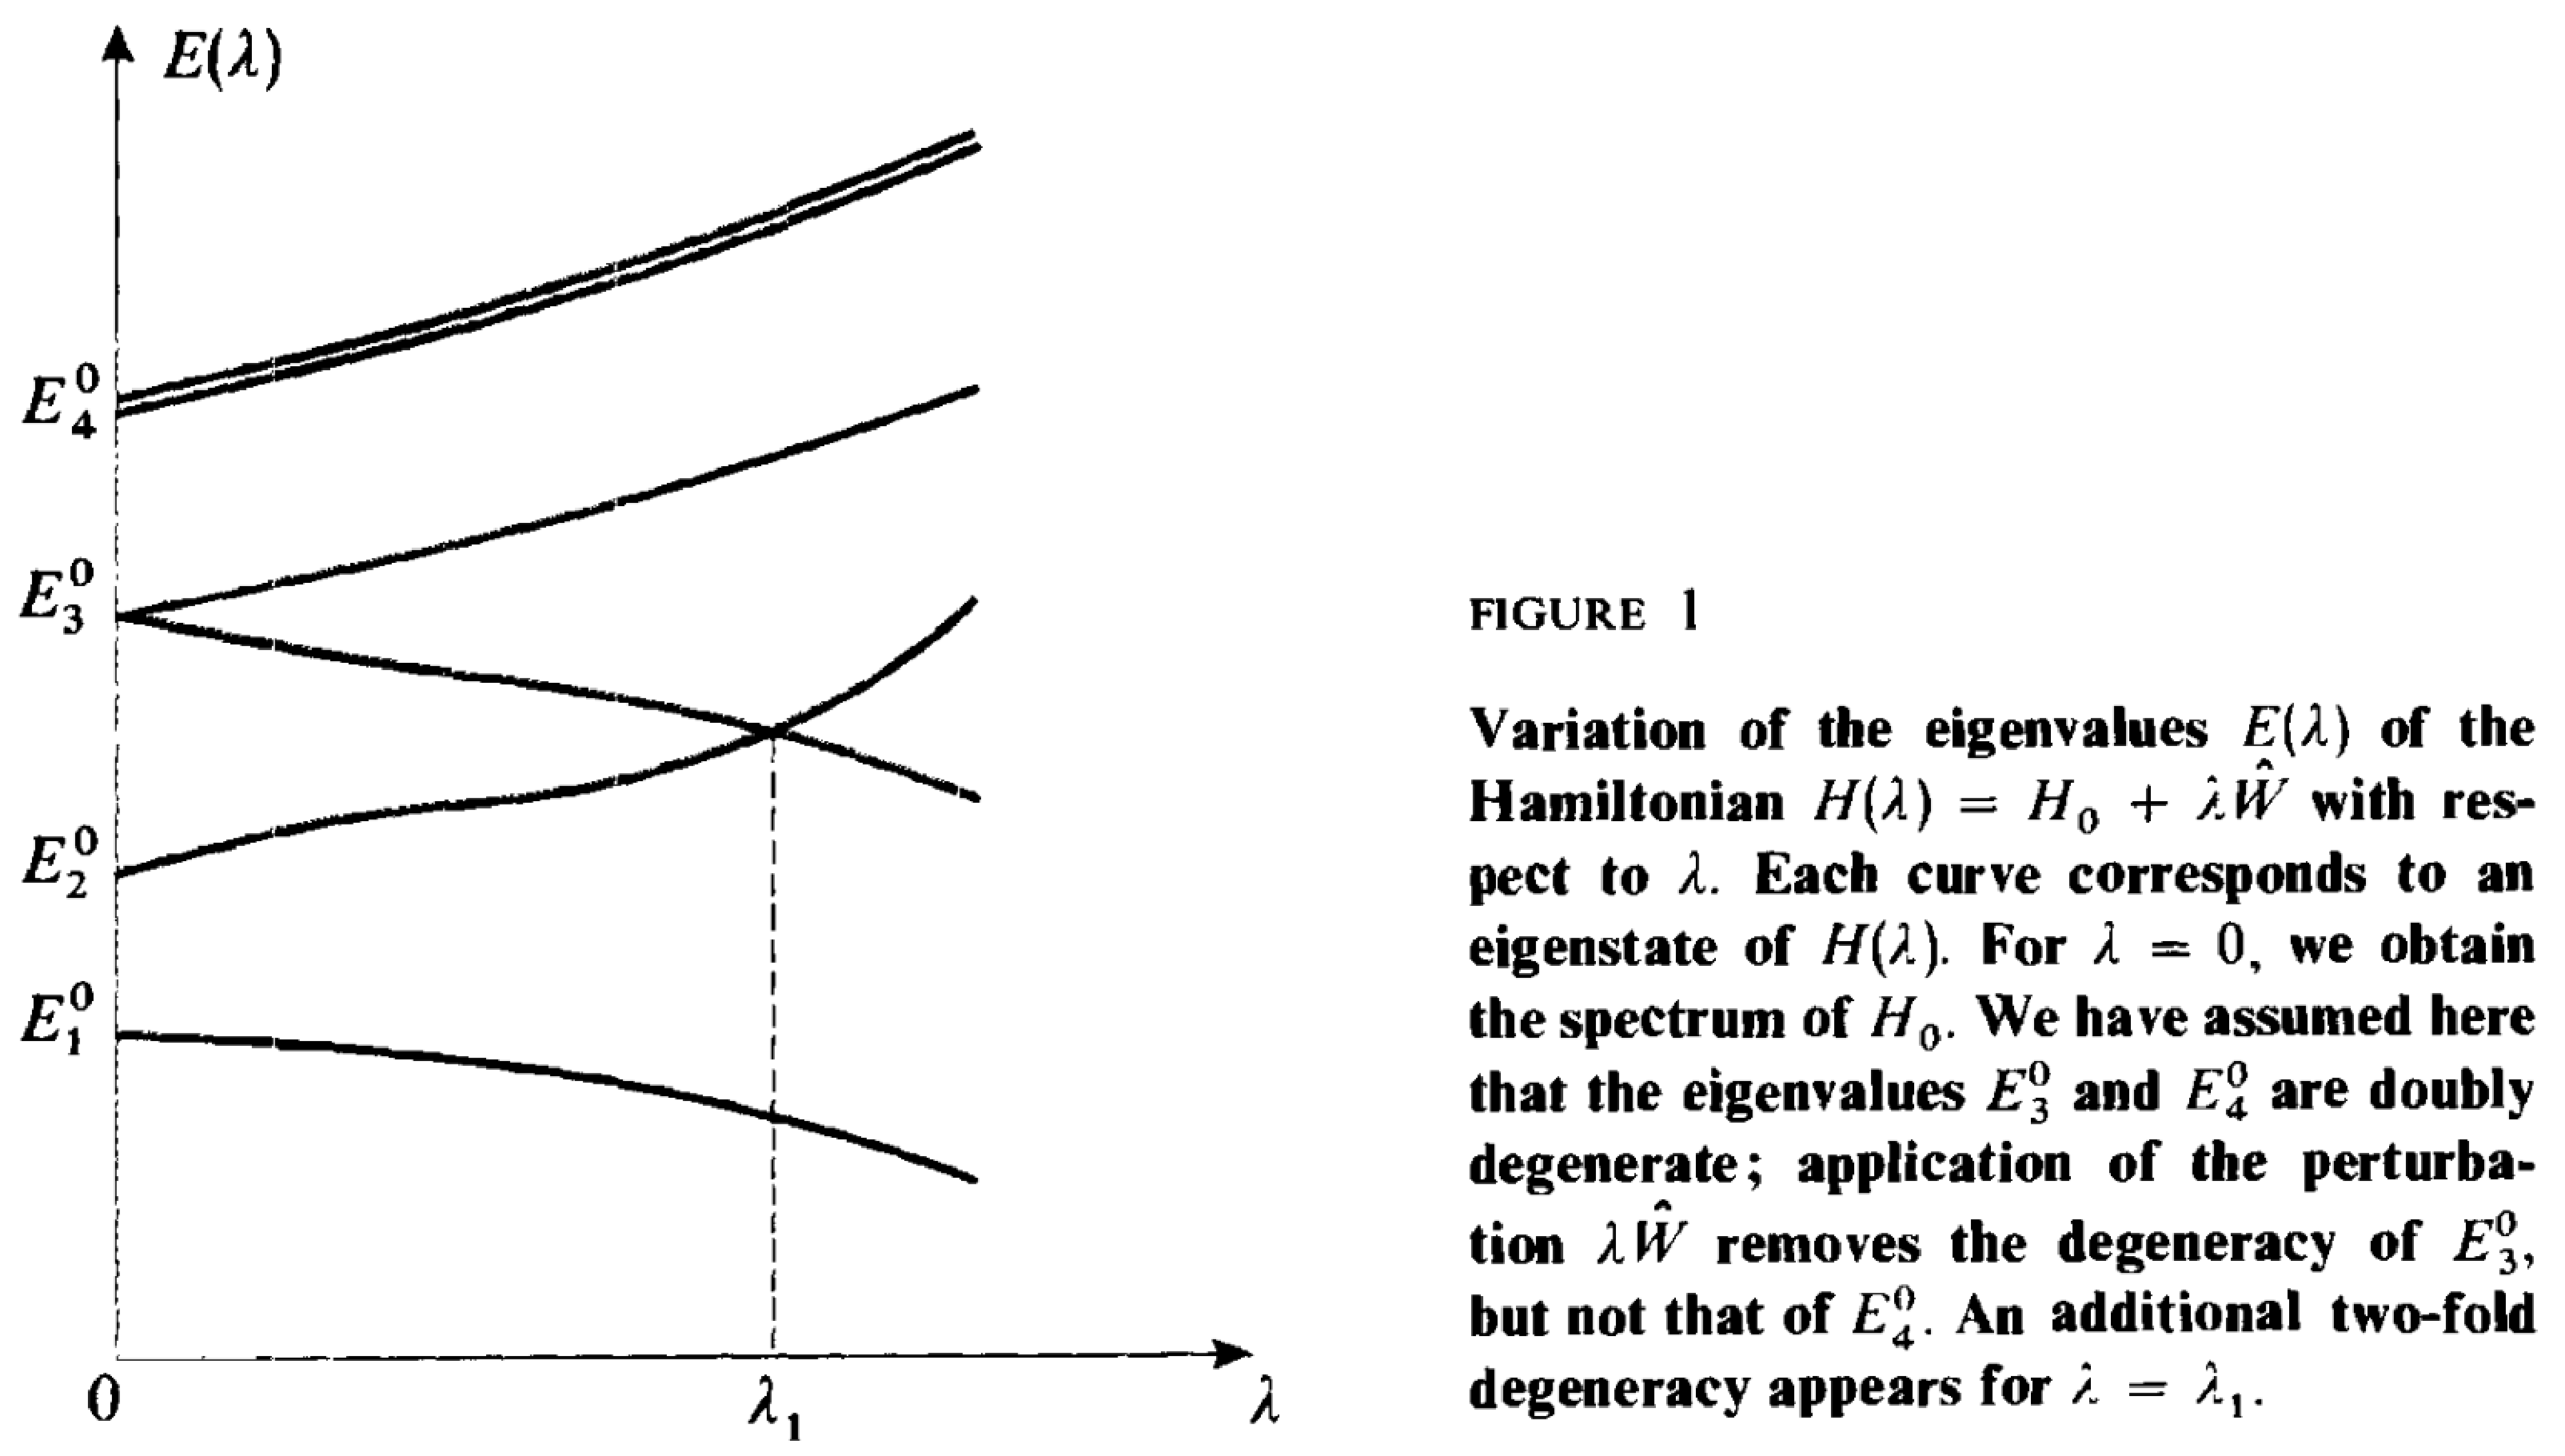
\includegraphics[keepaspectratio=true,scale=0.20]{imgs/ipotesi2.pdf}
	\captionof{figure}{}
	\label{fig:fig-ipotesi}
\end{figure} 

Si prosegue sostituendo la \reff{serie-generale-E} e la \reff{serie-generale-phi} nella \reff{sistema-icognito-full} dove $H$ è usata con la sua espressione, per ricavare le equazioni che forniscono i coefficienti $\varepsilon_l$ e $\ket{k}$:
\begin{small}
	\begin{equation}
	\label{sostituzione-serie}
	H_0 \sum_{k = 0}^{\infty} \ket{k} \lambda^k + V \sum_{k = 0}^{\infty} \ket{k} \lambda^{k-1} = \sum_{l = 0}^{\infty} \varepsilon_l \lambda^l \sum_{k = 0}^{\infty} \ket{k} \lambda^k = \sum_{l,k = 0}^{\infty} \varepsilon_l \ket{k} \lambda^{l+k}
	\end{equation}
\end{small}
Ponendo $l^{'} = k+l$ e ricordando che $\sum_{l,k} = \sum_{l'=0}^{\infty} \sum_{l = 0}^{l'}$, manipolando algebricamente la \reff{sostituzione-serie} si puo' arrivare a:
\begin{equation}
	\label{soluzione-serie}
	(H_0 - \varepsilon_0) \ket{N} - \sum_{j = 1}^{N-1} \varepsilon_N \ket{N-1} - \varepsilon_N \ket{0} + V \ket{N-1} = 0
\end{equation}
che con $N = 1, 2, 3, ...$ fornisce l'equazione N-esima per il termine correttivo N-esimo. L'equzione per $N=0$ si ottiene ricordando che nella \reff{sostituzione-serie} i coefficienti di ogni potenza di $\lambda$ devono eguagliarsi (metodo generale alternativo a \reff{soluzione-serie}). Si scrivono le equzione per $N = 0, 1, 2$:
\begin{equation}
	\label{ordine0}
	N = 0 \Rightarrow  H_0 \ket{0} = \varepsilon_0 \ket{0}
\end{equation}
\begin{equation}
\label{ordine1}
N = 1 \Rightarrow  (H_0 - \varepsilon_0) \ket{1} + (V - \varepsilon_1) \ket{0} = 0
\end{equation}
\begin{equation}
\label{ordine2}
N = 2 \Rightarrow  (H_0 - \varepsilon_0) \ket{2} + (V - \varepsilon_1) \ket{1} -  \varepsilon_2 \ket{0}
\end{equation}

La \reff{ordine0} dice che $\varepsilon_0$ è autovalore di $H_0$ con autostato $\ket{0}$, esiste cioè $E_n^{(0)}$ unico t.c. $\varepsilon_0 = E_n^{(0)}$. L'insieme dei $\ket{\phi(\lambda)}$ corrispondenti alle energie $E(\lambda)$ che tendono al livello fissato $E_n^{(0)}$ per $\lambda \to 0$, formano un sottospazio di stati. Si suppone (ipotesi verosimile) che per $\lambda \to 0$ la dimensione del sottospazio vari con continuità con $\lambda$. Segue che la dimensione dello spazio è pari alla degenerazione $g_n$ del particolare livello energetico considerato $E_n^{(0)}$. Quindi nel caso $E_n^{(0)}$ non fosse degenere, avrebbe associata un'unica energia $E(\lambda)$ anche essa non degenere.

A questo punto, si continua lo sviluppo del metodo perturbativo, considerando il caso specifico in cui lo spettro di $H_0$ non è degenere.

%%
\section{Spettro non degenere}
Si suppone che la \reff{sistema-noto-full} non abbia energie degeneri, in questo la caso si può riscrivere come:
\begin{equation}
	\label{noto-non-degenere}
	H_0\ket{\phi_{n}^{(0)}} = E_n^{(0)}\ket{\phi_{n}^{(0)}}
\end{equation}
Vale quindi $g_n = 1$, e per quanto detto sopra, risulterà che $E(\lambda)$ non e' degenere. Sia $\varepsilon_0 = E_n^{(0)}$, risulta dalla \reff{ordine0} che $\ket{0}$ è proporzionale a $\ket{\phi_n^{(0)}}$. Siccome $\ket{\phi_n^{(0)}}$ è definito a meno di una costante, ricordando che si supponongono entrambi normalizzati (vedi \reff{reale-icognito}), si può scegliere arbitrariamente la fase in modo che per $\lambda \to 0$.
\begin{equation}
	\label{espressione-stato0}
	\ket{0} = \ket{\phi_n^{(0)}}
\end{equation}

Quindi i termini correttivi all'ordine zero sono dati dagli autovalori ed autostati del sistema noto che è quello che ci aspettava avendo supposto che per $\lambda = 0, H = H_0$.

Vale la pena ricavare i termini all'ordine $N = 1$ in quanto è un risultato importante e molto usato per risolvere sistemi fisici reali. Si indicherà con $E_n(\lambda)$ l'autovalore di $H(\lambda)$ che tende a $E_n^{(0)}$ per $\lambda \to 0$. Si suppone inoltre che $\lambda$ sia abbastanza piccolo di modo che $E_n(\lambda)$ non sia mai degenere (usando l'esempio della figura \reff{fig:fig-ipotesi}: $\lambda << \lambda_1$), in questo caso si indicherà con $\ket{\phi_n(\lambda)}$ il relativo autostato associato.

Per calcolare $\varepsilon_1$ si inizia proiettando la \reff{ordine1} su $\ket{\phi_n^{(0)}}$:
\begin{equation}
	\label{ordine1-energia-proiezione}
	\bra{\phi_n^{(0)}}(H_0 - \varepsilon_0) \ket{1} + \bra{\phi_n^{(0)}}(V - \varepsilon_1)\ket{0} = 0
\end{equation}
Sostituendo $\ket{0} = \ket{\phi_{n}^{(0)}}$, $\varepsilon_0 = E_n^{(0)}$, usando la \reff{normalizzazione} e la \reff{noto-non-degenere} e ricordando che $H_0$ è un'operatore hermitiano, si puo' riscrivere:
\begin{equation}
	\label{ordine1-energia-proiezione2}
	E_n^{(0)}\braket{\phi_n^{(0)} | 1} - E_n^{(0)}\braket{\phi_n^{(0)} | 1} + \braket{\phi_n^{(0)}|V|\phi_n^{(0)}} - \varepsilon_1 \braket{\phi_n^{(0)}|\phi_n^{(0)}} = 0
\end{equation}
da cui si ricava:
\begin{equation}
	\label{energia1}
	\varepsilon_1 = \braket{\phi_n^{(0)}|V|\phi_n^{(0)}}
\end{equation}
Che dice che la correzione al primo ordine dell'energia perturbata è pari al valore medio della perturbazione $V$ rispetto allo stato imperturbato $\ket{\phi_n^{(0)}}$. Il risutalto trovato è una delle equazioni piu' usate in quantistica quindi vale la pena ricordarlo.

Si ricava ora la correzione $\ket{1}$ all'ordine $N = 1$ dello stato perturbato. Si proietta la $\reff{ordine1}$ su tutti gli autostati $\ket{\phi_{p}^{(0)}}$. L'operazione equivale a rappresentare $\ket{1}$ nella base (ortonormale e completa) $\ket{\phi_{p}^{(0)}}$:
\begin{equation}
	\label{ordine1-vettore-proiezione}
	\bra{\phi_p^{(0)}}(H_0 - E_n^{(0)}) \ket{1} + \bra{\phi_n^{(0)}}(V - \varepsilon_1)\phi_n^{(0)} = 0
\end{equation}
usando le stesse considerazioni fatte per ricavare \reff{ordine1-energia-proiezione2} si puo' riscrivere:
\begin{equation}
	\label{ordine1-vettore-proiezione2}
	(E_p^{(0)} - E_n^{(0)}) \braket{\phi_p^{(0)} | 1} + \braket{\phi_p^{(0)} | V | \phi_n^{(0)}} - \varepsilon_1 \braket{\phi_p^{(0)} | \phi_n^{(0)}} = 0
\end{equation}
Una prima osservazione è che $ \braket{\phi_p^{(0)} | \phi_n^{(0)}} = 0$ per $p \ne n$. Si noti che se $\ket{1}$ è soluzione della \reff{ordine1} allora lo è anche $\ket{1} + \alpha \ket{0} = \ket{1} + \alpha \ket{\phi_{n}^{(0)}}$ per qualunque $\alpha$. Si può sempre sottrarre $\alpha\ket{\phi_{n}^{(0)}}$ dalla rappresentazione di $\ket{1}$ senza perdere di generalità. Si pone quindi $p \ne n$ nella \reff{ordine1-energia-proiezione2} e si ottiene:
\begin{equation}
	\label{ordine1-vettore-proiezione3}
	\braket{\phi_p^{(0)} | 1} = \frac{\braket{\phi_p^{(0)} | V | \phi_n^{(0)}}}{(E_n^{(0)} - E_p^{(0)}) }
\end{equation}

A questo punto, per avere la rappresentazione completa di $\ket{1}$, bisogna conoscere $\braket{\phi_n^{(0)} | 1}$. Il ragionamento e' analogo a quanto gia' detto per derivare la \reff{espressione-stato0}: in generale $\ket{\phi(\lambda)}$ è definito a meno di una costante, e quindi si possono scegliere arbitrariamente norma e fase. In questo caso si sceglie
\begin{equation}
	\label{normalizzazione-incognito}
	\braket{\phi(\lambda) | \phi(\lambda)} = 1
\end{equation}
mentre la convenzione adottata per la fase varia in funzione del manuale cosultato: ad esempio il Messiah\cite{messiah} richiede $\braket{0 | \phi(\lambda)} = \braket{0 | 0} = 1$ che poi implica $\braket{0 | k} = 0$ con $k = 1, 2, ...$ . Il Cohen\cite{cohen} invece rilassa l'ipotesi richiedendo $\braket{0 | \phi(\lambda)} \in \Re$. Questa ipotesi ovviamente non fissa la fase, che quindi andrà scelta di volta in volta.

L'utilità della convenzione scelta dipende dall'ordine dello sviluppo che si sceglie. In ogni caso, l'ipotesi $\braket{0 | \phi(\lambda)} \in \Re$ implica $\braket{0 | 1} = \braket{0 | 1} = 0$, quindi in questo caso, all'ordine $N=1$, l'ipotesi scelta è indifferente. Nel resto del testo si sceglie l'ipotesi piu' generale:
\begin{equation}
	\label{reale-icognito}
	\braket{0 | \phi(\lambda)} \in \Re
\end{equation}

Siccome si può dimostrare che \reff{reale-icognito} implica $\braket{0 | 0} = 1$ e $\braket{0 | 1} = \braket{0 | 1} = 0$, allora si può dire che la \reff{ordine1-vettore-proiezione2} e' la rappresentazione esatta di $\ket{1}$, e quindi si può scrivere:
\begin{equation}
	\label{stato1}
	\ket{1} = \sum_{p \ne n} \frac{\braket{\phi_p^{(0)} | V | \phi_n^{(0)}}}{(E_n^{(0)} - E_p^{(0)}) } \ket{\phi_{p}^{(0)}}
\end{equation}

Secondo i risultati trovati, i termini perturbati, si possono scrivere al primo ordine come:
\begin{equation}
	\label{soluzione1-energia}
	E_n(\lambda) = E_n^{(0)} + \braket{\phi_n^{(0)}|V|\phi_n^{(0)}} + O(\lambda^2)
\end{equation}
\begin{equation}
\label{soluzione1-stato}
\ket{\phi_n(\lambda)} = \ket{\phi_n^{(0)}} + \sum_{p \ne n} \frac{\braket{\phi_p^{(0)} | \lambda V | \phi_n^{(0)}}}{(E_n^{(0)} - E_p^{(0)}) } \ket{\phi_{p}^{(0)}} + O(\lambda^2)
\end{equation}

Si noti che la \reff{soluzione1-stato} è correttamente definita perchè siccome si è supposto che non ci siano livelli energetici degeneri, allora se $p \ne n$ anche $E_n^{(0)} \ne E_p^{(0)}$.

Un'altra considerazione importante è che ora si può quantificare meglio l'ipotesi fatta inzialmente richiedendo che il termine perturbativo $\lambda V$ fosse piccolo rispetto ad $H_0$. Intanto, l'ipotesi $\lambda << 1$ implica che gli elementi della matrice associata a $V$ siano dello stesso ordine di quelli di $H_0$. La \reff{soluzione1-stato} permette di essere più precisi, infatti quello che risulta è che gli elementi della matrice $\lambda V$ devono essere molto più piccoli della differenza fra le energie al denominatore: $|(\lambda V)_{np}| << |E_n^{(0)} - E_p^{(0)}|$.

Una considerazione finale: il metodo sviluppato è iterativo. Questo significa che è possibile implementare un algoritmo che approssimi numericamente il sistema perturbato fino ad un grado $N$ arbitrario. Questa caratteristica è importante perchè in quantistica una buona parte dei problemi viene risolta proprio con l'analisi numerica. 

\begin{thebibliography}{}
	\bibitem[1]{cohen} Cohen-Tannoudji C., Diu B., Laloe F. - Quantum mechanics Volume 2(1996)
	\bibitem[2]{messiah} Albert Messiah - Quantum Mechanics
	\bibitem[3]{griffith} David J. Griffiths, Darrell F. Schroeter - Introduction to quantum mechanics 3rd edition
	\bibitem[4]{dirac} P. A. M. DIRAC - The principles of quantum mechanics 3rd edition (letto solo in modo qualitativo)	  
\end{thebibliography}


\end{document}
